\documentclass[10pt,a4paper,twocolumn]{article}

\usepackage[T1]{fontenc}
\usepackage[utf8]{inputenc}
\usepackage{lmodern}
\usepackage[a4paper,margin=2cm,columnsep=0.6cm]{geometry}
\usepackage{graphicx}
\usepackage{booktabs}
\usepackage{amsmath}
\usepackage{siunitx}
\usepackage[font=small,labelfont=bf]{caption}
\usepackage[round,authoryear]{natbib}
\usepackage[hidelinks]{hyperref}

\sisetup{separate-uncertainty=true, range-phrase={ to }, per-mode=symbol}
\graphicspath{{figures/}}

\title{Inflation Cycles at Svartsengi, Iceland:\\ GNSS--InSAR Comparison and Source Stability}
\author{Cai Zhihao, Raúl Lara, Génio Lay da Silva, Diogo Correia, Otto Scipal\\
\small Space Geodesy, Institute of Geodesy and Photogrammetry, ETH Zurich}
\date{}

\begin{document}

\twocolumn[
\begin{@twocolumnfalse}
\maketitle
\begin{abstract}
Since November 2023, magma accumulation beneath Svartsengi, Iceland, has caused repeated cycles of uplift, each ended by a dike intrusion or an eruption at the Sundhnúkur crater row; no eruption has occurred since August 2025. This study asks how the uplift rate changed across the cycles and during the current pause, how well InSAR agrees with GNSS during this fast deformation, and whether the spatial pattern of uplift stayed the same. LiCSAR interferograms of two Sentinel-1 frames were inverted into time series with LiCSBAS and decomposed into vertical and east components; 14 GNSS stations served for validation and rates. The uplift rate fell in steps from $11.4 \pm 1.2$~mm/day after the first intrusion to about 4~mm/day in 2024 and 2.6~mm/day in 2025. During the pause it declined continuously, to $0.39 \pm 0.05$~mm/day at station SENG by October 2026. Over inflation periods InSAR and GNSS agree within 15 to 20~mm and 0.2~mm/day, while across the intrusions they differ by hundreds of millimetres near the dikes. Since March 2024 the centre of the uplift moved by less than 90~m between cycles, and its extent and shape stayed the same.
\end{abstract}
\vspace{1em}
\end{@twocolumnfalse}
]

\begin{figure*}[t]
  \centering
  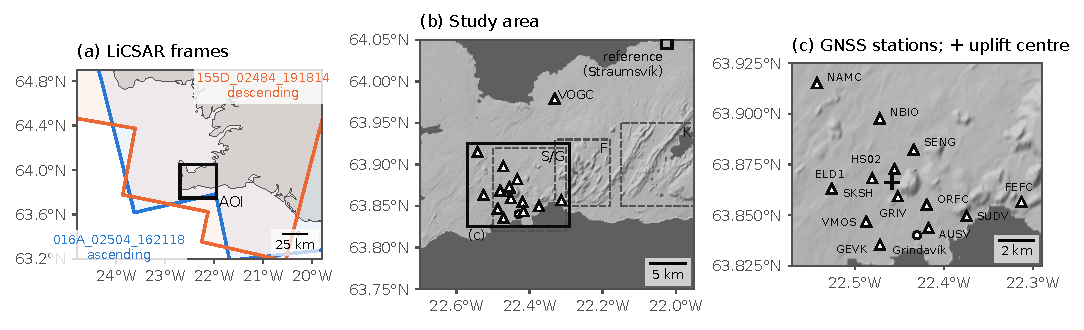
\includegraphics[width=\textwidth]{fig1_study_area.pdf}
  \caption{(a) Footprints of the LiCSAR frames and the processed area (AOI). (b) Processed area with the InSAR reference window at Straumsvík (square) and the areas with their own deformation (dashed; S/G Sundhnúkur and Grindavík, F Fagradalsfjall, K Krýsuvík), excluded when the reference was chosen. (c) GNSS stations (triangles), the nominal uplift centre (+) and Grindavík (circle).}
  \label{fig:area}
\end{figure*}

\section{Introduction}

After about 800 quiet years, inflation and deflation cycles resumed at Svartsengi on the Reykjanes Peninsula in 2020 \citep{flovenz2022,cubuk2021}. Uplift started again on 27 October 2023, and on 10 November 2023 a 15~km long dike formed beneath Grindavík \citep{sigmundsson2024,depascale2024}. Until July 2025, 11 dike intrusions and 9 eruptions followed along the Sundhnúkur crater row \citep{parks2025,parks2026}. In each cycle magma accumulates at 4 to 5~km depth beneath Svartsengi and the ground rises, until a dike propagates towards the crater row and the ground subsides within hours. No eruption has occurred since August 2025, although accumulation continued \citep{imo2026}; a declining magma supply or a changed stress state in the crust are possible explanations \citep{parks2026}, and both would show in the rate and pattern of surface deformation.

GNSS gives daily three dimensional positions at single points, while Sentinel-1 InSAR maps the displacement of a whole area in the line of sight (LOS) every 6 or 12 days \citep{torres2012}. Interferograms from the COMET LiCSAR service \citep{lazecky2020} can be inverted into time series with LiCSBAS \citep{morishita2020}, but metre scale displacements at dikes and new lava cause unwrapping errors and coherence loss \citep{hanssen2001}.

Following the research plan, this study asks (1) how the uplift rate changed across the inflation cycles since October 2023 and during the current pause, (2) how well InSAR time series agree with GNSS during rapid volcanic deformation, and (3) whether the spatial pattern of uplift remained stable between cycles. No source model is fitted and no volumes are derived.

\section{Data}

\textbf{InSAR.} All LiCSAR interferograms since January 2020 of the ascending frame \texttt{016A\_02504\_162118} (3747, until 16 September 2026) and the descending frame \texttt{155D\_02484\_191814} (1591, until 3 February 2026, the last processed product) were used (Fig.~\ref{fig:area}a). Products that need both geometries therefore end on 3 February 2026. They are geocoded on a 0.001$^\circ$ grid (about 111 by 49~m) and were cut to \ang{22.70}W to \ang{21.95}W, \ang{63.75}N to \ang{64.05}N. GACOS weather model corrections \citep{yu2018} exist for all epochs. LiCSAR contains modified Copernicus Sentinel data 2020 to 2026 analysed by the Centre for the Observation and Modelling of Earthquakes, Volcanoes and Tectonics (COMET).

\textbf{GNSS.} Daily IGS20 positions of all 14 stations within 15~km of the uplift centre were taken from the Nevada Geodetic Laboratory \citep{blewitt2018} (Fig.~\ref{fig:area}c). Only SKSH and SENG cover the full period; most others start in November 2023 or later. The data end in May 2026, for SENG, AUSV, GEVK and VOGC in October 2026. Station REYK in Reykjavík, 39~km from the centre, served as reference.

\begin{figure*}[t]
  \centering
  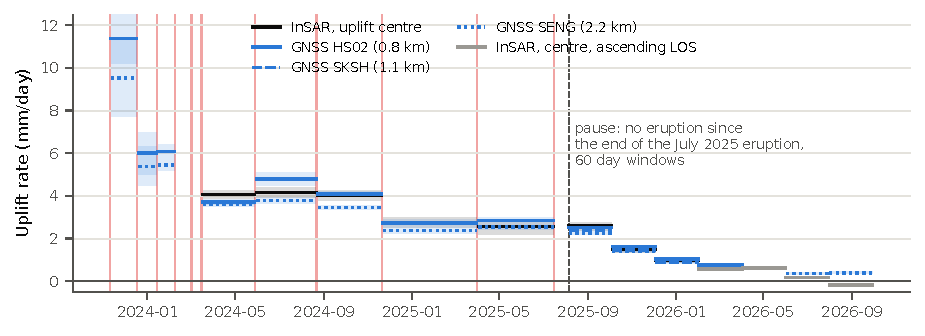
\includegraphics[width=\textwidth]{fig_rates.pdf}
  \caption{Vertical uplift rate per inflation period since October 2023 (segments, shading $\pm 1\sigma$), from InSAR at the uplift centre and GNSS at the three nearest stations (distance to the centre). Right of the dashed line: the current pause in 60 day windows; grey: ascending LOS rate at the centre after the vertical component ends. Red lines: dike intrusions and eruptions.}
  \label{fig:rates}
\end{figure*}

\section{Methods}

\textbf{InSAR time series.} The interferograms were processed with the COMET version of LiCSBAS \citep{morishita2020}. GACOS corrections were subtracted and interferograms with low coherence were removed. With the default loop closure threshold of 1.5~rad, all ten descending interferograms across the intrusion of 10 November 2023 were rejected, which split the network and lost the step, although the loop errors were concentrated at the dike. The descending threshold was therefore raised to 3~rad, and pixels whose loops all fail were removed per interferogram (option \emph{nullify}). After the inversion, pixels with too many interferograms outside closed loops were masked. Both frames are referenced to the most coherent $5 \times 5$ pixel window at least 24~km from the centre and outside the active areas, at Straumsvík (\ang{64.046}N, \ang{22.024}W; Fig.~\ref{fig:area}b). With two geometries and the north component neglected, the vertical and east displacement follow from a $2 \times 2$ system per pixel \citep{wright2004}, with the ascending series interpolated to the descending epochs, never across an event. The nominal uplift centre (\ang{63.866}N, \ang{22.458}W) is the peak of the vertical displacement in several inflation periods; point series are $3 \times 3$ pixel means of the unfiltered series.

\textbf{GNSS.} Positions were taken relative to REYK, which removes plate motion and common errors. Offsets at antenna changes were estimated with a line and a step within 15 days. Outliers were removed against a 15 day running median, with a threshold of five times the robust standard deviation; the series is split at every event, and the first 10 days after each event are not tested, because the ground moves fast then. This removed 0.1 to 5~\% of the days per station and component.

\textbf{Uplift rates (question 1).} Event dates were taken from \citet{parks2025}, \citet{parks2026} and the Icelandic Meteorological Office. An inflation period runs from 2 days after one event to 1 day before the next. Its rate is the slope of a line fitted to all GNSS days or InSAR epochs in it. The standard deviation from the residuals is multiplied by $\sqrt{(1+\rho)/(1-\rho)}$, with $\rho$ the lag one autocorrelation of the residuals, because daily GNSS noise is correlated and the uplift within a period is not exactly linear. Periods shorter than 20 days, GNSS with data on less than 60~\% of the days and InSAR with fewer than four epochs get no rate. The pause, from 6 August 2025, was split into 60 day windows.

\textbf{InSAR and GNSS (question 2).} GNSS displacements were projected onto the LOS of each frame and compared with InSAR at the InSAR epochs, as whole series and as the change over each inflation period and each event; the InSAR rates were also computed at the station pixels.

\textbf{Uplift pattern (question 3).} For every cycle, the vertical displacement between its first and last epoch within 7~km of the nominal centre was fitted with an elliptical Gaussian surface plus a constant, which gives the centre, the half maximum ellipse as measure of the extent, and its orientation. As the residuals are spatially correlated, the formal errors were scaled with the number of independent pixels, the fitted area divided by $\pi L^2$, where $L$ (0.8 to 1.6~km) is the distance at which the autocorrelation of the residual map falls to $1/e$. The shape was compared by the correlation coefficient between each map and the mean of the amplitude normalised maps of all other cycles since 2023.

\begin{table}[t]
  \centering
  \caption{Vertical uplift rate in mm/day ($\pm 1\sigma$) per inflation period (start date) and in the 60 day windows of the pause, from InSAR at the centre and GNSS at HS02 (0.8~km) and SENG (2.2~km). Dash: no rate (period too short, too few epochs or no data).}
  \label{tab:rates}
  \footnotesize
  \setlength{\tabcolsep}{4pt}
  \begin{tabular}{@{}lrrr@{}}
    \toprule
    Period & InSAR centre & GNSS HS02 & GNSS SENG \\
    \midrule
    2023-11-12 & -- & $11.39 \pm 1.17$ & $9.54 \pm 1.81$ \\
    2023-12-20 & -- & $6.00 \pm 0.98$ & $5.38 \pm 0.91$ \\
    2024-01-16 & -- & $6.08 \pm 0.31$ & $5.45 \pm 0.27$ \\
    2024-03-18 & $4.05 \pm 0.20$ & $3.72 \pm 0.13$ & $3.60 \pm 0.11$ \\
    2024-05-31 & $4.16 \pm 0.22$ & $4.79 \pm 0.30$ & $3.78 \pm 0.13$ \\
    2024-08-24 & $4.01 \pm 0.24$ & $4.08 \pm 0.12$ & $3.45 \pm 0.10$ \\
    2024-11-22 & $2.74 \pm 0.24$ & $2.73 \pm 0.17$ & $2.38 \pm 0.12$ \\
    2025-04-03 & $2.56 \pm 0.35$ & $2.84 \pm 0.15$ & $2.53 \pm 0.11$ \\
    \midrule
    \multicolumn{4}{@{}l}{Pause, windows starting} \\
    2025-08-06 & $2.58 \pm 0.18$ & $2.51 \pm 0.06$ & $2.25 \pm 0.06$ \\
    2025-10-05 & $1.51 \pm 0.14$ & $1.62 \pm 0.04$ & $1.39 \pm 0.06$ \\
    2025-12-04 & $0.96 \pm 0.10$ & $1.03 \pm 0.07$ & $0.92 \pm 0.05$ \\
    2026-02-02 & -- & $0.76 \pm 0.07$ & $0.68 \pm 0.05$ \\
    2026-04-03 & -- & -- & $0.62 \pm 0.05$ \\
    2026-06-02 & -- & -- & $0.36 \pm 0.05$ \\
    2026-08-01 & -- & -- & $0.39 \pm 0.05$ \\
    \bottomrule
  \end{tabular}
\end{table}

\begin{figure*}[t]
  \centering
  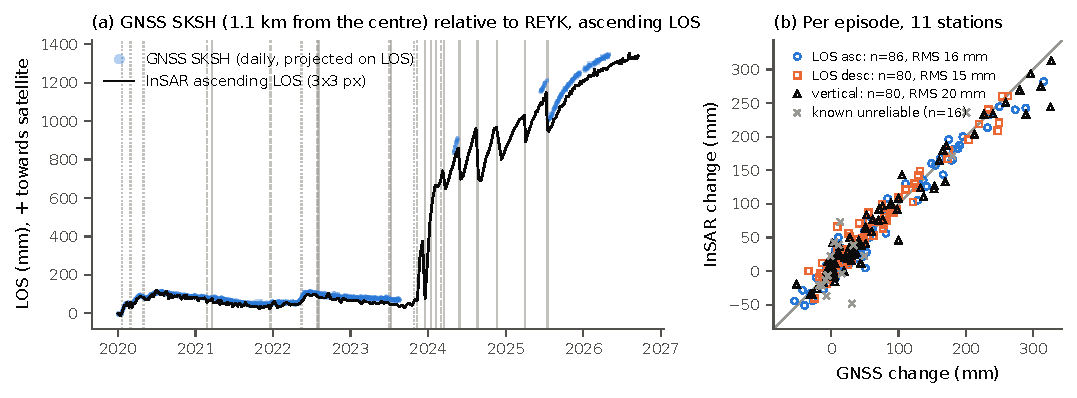
\includegraphics[width=\textwidth]{fig6_gnss_comparison.pdf}
  \caption{(a) Ascending LOS at SKSH: InSAR ($3 \times 3$ pixels) and daily GNSS projected onto the LOS, both relative to their references. (b) Change over each inflation period, InSAR against GNSS, for all stations with data on both epochs; crosses mark pairs affected by the known problems at the dikes.}
  \label{fig:gnss}
\end{figure*}

\section{Results}
\label{sec:results}

\textbf{(1) Uplift rate.} The uplift rate decreased in steps (Fig.~\ref{fig:rates}, Table~\ref{tab:rates}). At HS02 it fell from $11.39 \pm 1.17$~mm/day after the first intrusion to about 6~mm/day in December 2023 and January 2024. In the three cycles from March to November 2024 the rate at the centre stayed at 4.0 to 4.2~mm/day, the same within the uncertainties, and dropped to $2.74 \pm 0.24$ and $2.56 \pm 0.35$~mm/day in the two cycles before July 2025. Every cycle from March 2024 to July 2025 added 235 to 325~mm of uplift at the centre. During the pause the rate declines from window to window, at all stations and in InSAR: at HS02 from $2.51 \pm 0.06$~mm/day in August and September 2025 to $0.76 \pm 0.07$~mm/day in February and March 2026. At SENG, the only nearby station with data after May 2026, it reached $0.36 \pm 0.05$ and $0.39 \pm 0.05$~mm/day from June to October 2026, still above zero; the ascending LOS rate at the centre, $-0.18 \pm 0.28$~mm/day in August and September 2026, cannot resolve this.

\textbf{(2) InSAR and GNSS.} At SKSH, 1.1~km from the centre, InSAR follows GNSS in ascending LOS with 23~mm RMS difference over six years (Fig.~\ref{fig:gnss}a). Over the inflation periods, the changes at 11 stations differ by 16~mm RMS in ascending LOS ($n = 86$), 15~mm in descending LOS ($n = 80$) and 20~mm vertical ($n = 80$) (Fig.~\ref{fig:gnss}b). The InSAR rates at the station pixels are on average 0.18~mm/day (5 to 7~\%) lower than GNSS at HS02 and SENG, at most $0.74 \pm 0.37$~mm/day at HS02 from May to August 2024. Across the intrusions and eruptions the RMS difference is 15~mm in descending LOS, but 57~mm vertical, 75~mm east and 93~mm in ascending LOS, dominated by stations near the dikes. The step of 10 November 2023 is not recovered at SENG, SKSH, HS02, SUDV and FEFC (350 to 760~mm in descending LOS), and in Grindavík (AUSV) InSAR does not follow GNSS.
\begin{figure*}[t]
  \centering
  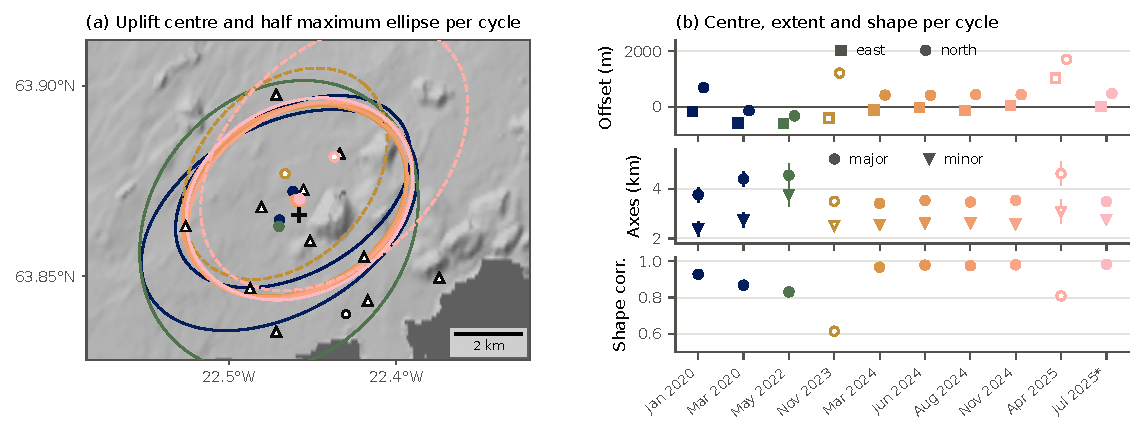
\includegraphics[width=\textwidth]{fig_pattern.pdf}
  \caption{Uplift pattern per cycle from Gaussian fits to the vertical displacement maps. (a) Fitted centres ($\pm 1\sigma$) and half maximum ellipses, coloured by time; open symbols and dashed: cycles affected by deformation along the dikes. (b) Offset of the centre from the nominal centre (+ in a), half maximum axes, and correlation of the shape with the other cycles since 2023. Jul 2025*: pause, until 3 February 2026.}
  \label{fig:pattern}
\end{figure*}

\textbf{(3) Uplift pattern.} All cycles show an elliptical uplift west of the Sundhnúkur crater row, elongated towards north east (Fig.~\ref{fig:pattern}). In the four cycles from March 2024 to March 2025 and in the pause, the centre lies at \ang{63.870}N, \ang{22.459}W, and the single centres are at most 89~m from their mean, with $1\sigma$ of 50 to 90~m. The half maximum axes are 3.41 to 3.53~km and 2.56 to 2.76~km (about $\pm 0.1$~km), the major axis points to 58 to \ang{62}, and the shape correlation is 0.97 to 0.98. The ten times smaller uplift of 2020 and 2022 has centres 0.29, 0.79 and 0.94~km ($\pm 0.2$~km) from the recent centre, the latter two to the south west, wider ellipses (major axes 3.8 to 4.5~km) and shape correlations of 0.83 to 0.93. Two cycles deviate: November 2023 (centre 0.86~km to the north, correlation 0.62) and April 2025 (1.66~km to the north east, correlation 0.81).

\section{Discussion}
\label{sec:discussion}

\textbf{Uplift rate.} The stepwise decrease agrees qualitatively with the decreasing inflow described by \citet{parks2025}. In the pause the rate keeps falling instead of staying constant as in 2024. Such a decay is expected if the inflow depends on the pressure difference to a deeper region while the pressure beneath Svartsengi keeps rising without an eruption, but a declining deep supply would look the same; surface rates alone cannot separate the two. The rate depends on the point: HS02 (0.8~km) rises up to 27~\% faster than SENG (2.2~km), so only rates at the same point should be compared over time.

\textbf{InSAR and GNSS.} During inflation InSAR is accurate enough for the rate trend; its small negative bias may come from the 300~m averaging and from the 11~km between the InSAR and GNSS references. GNSS remains necessary for the short cycles of late 2023 and early 2024, when the 12 day revisit gave too few epochs per period. The main limitation is the near field of the dikes, where metre scale gradients cannot be unwrapped over 50 to 110~m pixels and new lava reduces coherence. Raising the loop threshold kept the step in most of the descending series (median RMS difference to GNSS 87~mm before, 20~mm after), but not near the dikes.

\textbf{Uplift pattern.} Since March 2024 the uplift has kept its position, extent and shape within about 100~m, also in the pause until February 2026, so the surface pattern gives no sign of a change in the accumulation region. The 2020 and 2022 uplift lies slightly further south west, but its low amplitude makes the fit more sensitive to noise. The two deviating cycles are affected by other deformation: the November 2023 map spans only 24 days directly after the intrusion, with the dike zone decorrelated, and the April 2025 map starts 2 days after a dike that propagated north east, whose displacement pulls the fit. A stable surface pattern is necessary but not sufficient for a stable source, which would require modelling.

\textbf{Deviations from the research plan.} No dedicated Sentinel-1 processing was done; LiCSAR was sufficient during inflation, but own processing would have been needed for the dike steps and for descending data after 3 February 2026. For the reference the processed area was extended to the north east and the minimum distance raised to 24~km, the descending loop threshold was changed, and the uplift centre was taken from the data.

\section{Conclusions}

(1) The uplift rate fell in steps from $11.4 \pm 1.2$~mm/day in November 2023 to about 4~mm/day in 2024 and 2.6~mm/day in 2025, and since the last eruption it has declined continuously to $0.39 \pm 0.05$~mm/day at SENG by October 2026. (2) LiCSAR and LiCSBAS time series agree with GNSS within 15 to 20~mm and 0.2~mm/day during inflation, but not across the intrusions near the dikes. (3) Since March 2024 the uplift has been stable in centre, extent and shape.

\bibliographystyle{plainnat}
\bibliography{references}

\end{document}
